\section{Introduction}

Intensity Interferometry (II) was first reported by Hanbury Brown and Twiss (HBT) during the 1950s \citep{brown1954lxxiv, HBT56} as a \textquotedblleft new type of interferometry\textquotedblright\ to measure stellar parameters such as angular diameter, orbits, and limb darkening coefficients. Later, theoretical results reported by \cite{brown1957interferometry, brown1958interferometry}, along with those of \cite{glauber1963quantum} and others, demonstrated the deeper physical properties of photon correlations that lie at the core of II and laid the foundation for Quantum Optics \cite[for textbook treatments see][]{MandelWolf1995, Hecht2002}.

By the 1970s, with stellar parameter measurements of 32 stars in single and multiple star systems conducted by Hanbury Brown and his collaborators \citep{hanbury1974angular} at the historic Narrabri Stellar Intensity Interferometer (NSII) in Australia, II had emerged as an alternative to the already established technique of Michelson Interferometry for measuring stellar parameters. Despite these significant achievements, the method did not gain widespread adoption in the ensuing decades, primarily due to the unavailability of sensitive photon detectors and advanced data analysis equipment.

More recently, proposals to utilize Imaging Atmospheric Cherenkov Telescope (IACT) facilities for conducting II observations of stars have emerged\citep{LeBohec2006, nunez2010stellar, nunez2012high, 2013APh....43..331D}. It has been demonstrated that such observations could be carried out during bright, moonlit nights when $\gamma$-ray observations based on upper atmospheric Cherenkov showers were not feasible. This approach has the potential to enhance the scientific output of existing IACT facilities, and especially of the upcoming Cherenkov Telescope Array Observatory (CTAO).  SII observations at VERITAS, MAGIC, and HESS are now being reported \citep[e.g.,][]{2024ApJ...966...28A,2024MNRAS.529.4387A,2025MNRAS.537.2334V}. Simulations \citep[e.g.,][]{10.1093/mnras/stab2391, 10.1093/mnras/stac2433} have argued that recent advancements in photon detectors could be effective in achieving high-precision measurements of parameters for stellar objects. 

Beyond measuring stellar diameters and other parameters of star systems, a fundamental goal of optical astronomy is to image stellar systems at high angular resolution.  In the context of II, this involves reconstructing the source's image from the intensity correlations recorded by pairs of telescopes (light buckets) on the ground. However, because the primary observable in II is the intensity of electromagnetic field rather than the amplitude, the phase of the interferometric signal is lost. So, there is a challenge to recover the phase of the signal, since a complete reconstruction of a source's brightness distribution requires phase information.

Several theoretical and computational approaches for phase reconstruction with II have been proposed. \cite{gamo1963triple} introduced the concept of triple-intensity correlation, which \cite{goldberger1963use} subsequently applied in an experiment to observe scattered particles in microscopic systems. Sato conducted experiments to measure the diameter and phase of asymmetrical objects, suggesting that triple correlation could extend II to image stellar bodies \citep{sato1978imaging, sato1979computer, sato1981adaptive}. However, achieving a satisfactory signal-to-noise ratio (SNR) remained a significant challenge for this approach.

\cite{GerchbergSaxton1972} suggested an iterative method to determine the phase from the image and diffraction plane pictures. This method relies on accurate initial estimates and is vulnerable to slow convergence otherwise. \cite{Fienup1982} introduced a Hybrid Input-Output algorithm that incorporates feedback mechanisms to improve convergence rate and robustness, particularly in noisy environments.

Later, \cite{holmes2010two} proposed an alternative method that utilizes the Cauchy-Riemann relations to reconstruct 1-D images. They also extended the approach to 2-D images across a range of signal-to-noise (SNR) values. This algorithm was applied to simulated data of stellar objects using II, considering both existing and forthcoming Imaging Cherenkov Telescope Arrays (IACTs) with a large number of telescopes \citep{nunez2010stellar, nunez2012high, nunez2012imaging}. However, this method faces challenges related to computational complexity when attempting to generalize to higher dimensions.

\cite{Li2014} suggested a flexible iterative Regularization method that incorporates prior information (e.g., sparsity, smoothness, or non-negativity) to reduce the ill-posedness of the phase retrieval problem. This method is more robust against noise and stabilizes the solution against artefacts and spurious solutions. Nevertheless, it faces challenges regarding the choice of the regularization parameter, computational complexity, and sensitivity to the initial guess.

The Transport-of-Intensity Equation (TIE) method is a non-interferometric technique first proposed by \cite{Teague1983} that relates the intensity variations along the optical axis to the phase of the optical fields. This method enables phase retrieval from intensity measurements taken at multiple planes. \cite{Zhang2020} proposed a method to obtain a \textquotedblleft universal solution\textquotedblright\ to the TIE by employing a \textquotedblleft maximum intensity assumption\textquotedblright, thereby converting the TIE into a Poisson equation which is then solved iteratively. More recently, \cite{Kirisits2024} have explored hybrid methods that combine the TIE with other equations, such as the Transport of Phase Equation (TPE). These approaches leverage the strengths of both equations to improve phase retrieval accuracy. This method is universally applicable, as it works for arbitrarily shaped apertures, handles non-uniform illumination, and accommodates inhomogeneous boundary conditions. It guarantees convergence, although the speed of convergence depends on the quality of the initial guess, and the final results are influenced by the boundary conditions.

With non-linearity built into their architecture, artificial neural networks (ANNs) empowered by deep learning methods are promising for exploring the task of reconstructing images of stellar objects from ground-based observations. Convolutional Neural Networks (CNNs), with their specialized architecture for processing two-dimensional datasets, are a natural choice for image processing tasks. In astronomical image reconstruction projects, a common challenge is that the interferometric data are typically undersampled as well as noisy.  Therefore, the CNN architectures and deep learning methods employed must be capable of reliably learning both the global context of the training dataset and the local features within it. Among the various CNN architectures, U-Net models \citep{ronneberger2015u} have proven successful in such tasks.

Furthermore, given that achieving a high signal-to-noise ratio (SNR) is often challenging in astronomical datasets, it is immensely beneficial if additional data can be generated using the available information from the observed sky density distribution and ground-based observations (II data, in our case) of the sources under investigation. Generative Adversarial Networks (GANs), introduced by \cite{goodfellow2014generative}, have been successful in such data augmentation tasks. Conditional GAN (cGAN) architectures, proposed by \cite{mirza2014conditional} and applied to a wide variety of datasets by \cite{isola2017image}, leverage additional information about the images in the training datasets and have demonstrated remarkable robustness in image recovery across diverse data types.

In the astrophysical context, \cite{schawinski2017galaxypics} employed a GAN model to recover features — such as spiral arms, central bulges, and disk structures of galaxies — from noise-affected images. \cite{mustafa2019cosmogan} developed and customized a Deep Convolutional GAN, dubbed \textquotedblleft CosmoGAN\textquotedblright, capable of generating high-fidelity weak-lensing convergence maps of dark matter distribution that statistically reproduce real weak lensing structures. \cite{coccomini2021lightweightgan} have successfully generated credible images of planets, nebulae, and galaxies using \textquotedblleft lightweight\textquotedblright\ and \textquotedblleft physics-uninformed\textquotedblright\ GANs to produce synthetic images of celestial bodies. They also generated a \textquotedblleft Hubble Deep Field-inspired\textquotedblright\ wide-view simulation of the universe. 

In this paper, we propose a conditional Generative Adversarial Network (cGAN) model \citep[following][]{isola2017image} to reconstruct images of fast-rotating stars using their simulated Intensity Interferograms and simulated sky-intensity distributions as input data for training, testing, and validation. We consider four Imaging Cherenkov Telescope Arrays (IACTs) and simulate observation of a fast-rotating star. The image predicted by the trained GAN shows promising results in reconstructing the star’s shape and size. The reconstructed brightness distributions are then assessed using moments.

This paper is organized as follows. The next section discusses Intensity Interferometry, focusing on its signal and noise characteristics for fast-rotating stars along the Earth’s rotation. The following section introduces the GAN formulation and its structure. The fourth section details the parameter selection for training the GAN for image reconstruction. The fifth section presents the results of the trained GAN both visually and via image moments. Finally, the paper concludes with a discussion of the overall results.
\begin{figure}
	\centering
	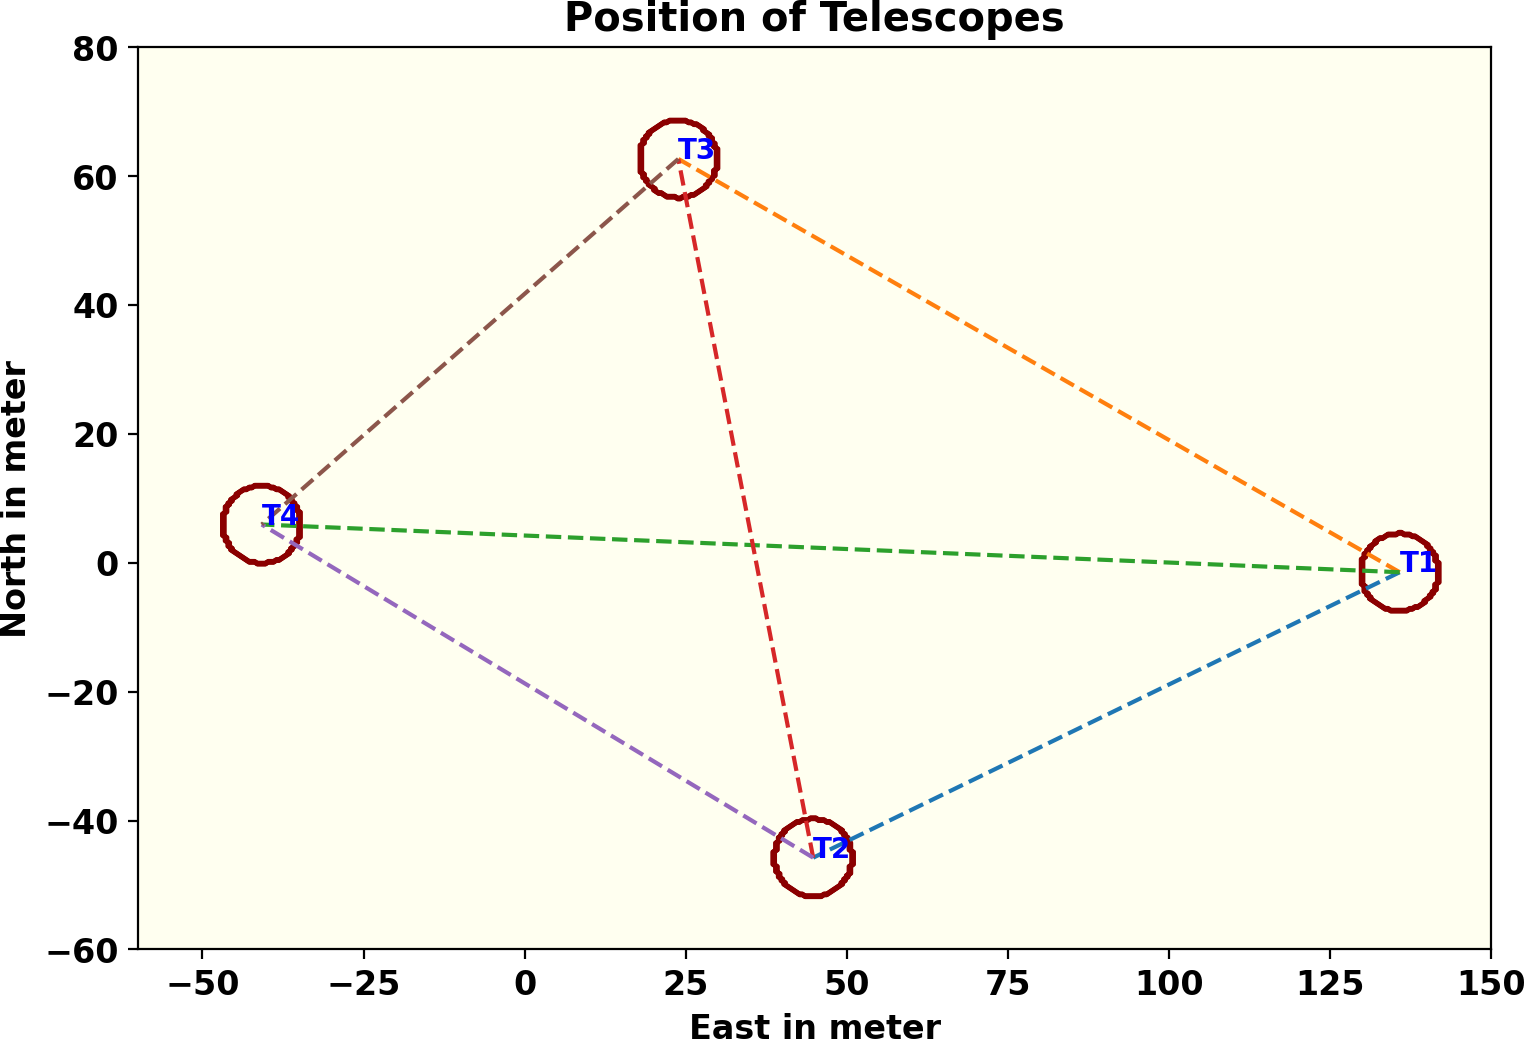
\includegraphics[width=\linewidth]{fig/telescope.png}
	\caption{The telescope configuration with similar properties each used to simulate the signal for II observation.}
	\label{fig:teles}
\end{figure}